\documentclass{beamer}
\usetheme{Szeged}
\usecolortheme{beaver}

\usepackage{listings}
\usepackage{color}
\usepackage{svg}
\usepackage{MnSymbol,wasysym}

\definecolor{pblue}{rgb}{0.13,0.13,1}
\definecolor{pgreen}{rgb}{0,0.5,0}
\definecolor{pred}{rgb}{0.9,0,0}
\definecolor{pgrey}{rgb}{0.46,0.45,0.48}

\usepackage{listings}
\lstset{language=Java,
  showspaces=false,
  showtabs=false,
  breaklines=true,
  showstringspaces=false,
  breakatwhitespace=true,
  commentstyle=\color{pgreen},
  keywordstyle=\color{pblue},
  stringstyle=\color{pred},
  basicstyle=\small
}


\begin{document}
\title{Dependency Injection}   
\author{Jonas Verhoelen} 
\date{\today} 

\frame{\titlepage} 

\frame{\frametitle{Table of contents}\tableofcontents} 

%% INTRODUCTION
\section{Introduction}
\frame{\frametitle{What you can expect}
\begin{itemize}
\item Theory about Dependency injection and connected topics
\item Examples to quickly understand the concepts
\item Tasks and exercises for the purpose of self-study
\end{itemize}
}

%% THEORY
\section{Theory} 
\frame{\frametitle{What is Dependency Injection?}
\begin{itemize}
\item Design pattern and concept in Object oriented programming
\item Way to get rid of hard-coded dependencies and replace by loose coupling
\item Moves the resolution of dependencies from compile-time to runtime
\item Very practical to create extendable and maintainable software, especially in big projects
\item Part of a lot of frameworks which take even more workload from you
\item ...something you \textbf{definitely have to} get familiar with!
\end{itemize}
}

%% EXAMPLE
\section{Example} 
\frame{\frametitle{Classic coupling (composition)}

\lstinputlisting[language=Java, firstline=1, lastline=20]{src/ServeOrderRunnable.java}
}

\frame{\frametitle{Classic coupling (aggregation) - explanation}

This was a minimal example for a simple aggregation between the classes ServeOrderRunnable and Restaurant. ServeOrderRunnable owns Restaurant but also other classes and objects can own it. The Restaurant is independent from ServeOrderRunnable and does not need it in order to be created or maintained.

\begin{center}
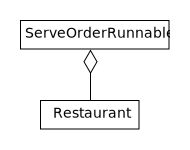
\includegraphics[scale=0.7]{img/aggregation.png}
\end{center}
}

\frame{\frametitle{Simplifying the situation - DI}
\lstinputlisting[language=Java, firstline=1, lastline=17]{src/ServeOrderRunnable_DI.java}
}

\frame{\frametitle{Simplifying the situation - DI2}

Huh? What happened?\\
We do not have to pass the Restaurant to the ServeOrderRunnable via the constructor anymore. The instance variable "restaurant" furthermore has a strange annotation above - @Autowired.\\
It's very simple: the annotation tells the application (based on Java Spring in this example) that this instance variable should be injected from the available services.

So:
\begin{itemize}
\item The class Restaurant is a service
\item @Autowired marks that this instance variable should be initialized with an object of the class Restaurant
\item A framework or self-written facility maintains instances of services and can inject them

\end{itemize}
}

\frame{\frametitle{Conclusion from the example}

Dependency Injection...

\begin{itemize}
\item makes dependencies the problems of someone else.
\item takes responsibilities from classes (less problems for you).
\item transfers responsibility to create, maintain and inject dependencies to one central mechanism.
\item is handled by a lot of frameworks so you can just use it out of the box without caring a lot.
\item also helps you testing, when complex dependencies are involved.
\end{itemize}
}

%% WORKSHOP
\section{Workshop} 
\frame{\frametitle{Get started}

This workshop contains a ready to go Java-application using the Spring framework. It lets you easily play around with Dependency Injection.

\begin{itemize}
\item Clone https://github.com/sebivenlo/dependency-injection.git
\item Open a command line and execute \textbf{cd workshop}
\item Execute \textbf{./gradlew build}
\item Execute \textbf{java -jar build/libs/gs-spring-boot-0.1.0.jar}
\end{itemize}

The server-app should run now. It is available under the URL localhost:8080/
Open the project in NetBeans now and see what happens. Feel free to play around.

}

\section{Workshop} 
\frame{\frametitle{Coffee machine task}

We want to build a coffee machine now in this application. The machine should have the following components:

\begin{itemize}
\item WaterContainer - contains water
\item WaterHeater - heats the water from the container
\item BeanContainer - contains coffee beans
\item BeanGrinder - grinds beans from the container
\item CoffeeMachine - the facade of a coffee machine, putting all components together
\end{itemize}

Construct a smart device out of these using the @Autowired and @Component annotations. When calling the app via its URL, it should make a coffee and print out the coffee on the site.
}


\frame{\frametitle{Coffee machine task - possible solution}

As always, there is more than one way to accomplish a task. In the repository you cloned, find the password-zipped \textbf{workshop-solution} folder (workshop-solution.zip).\\
Your lecturer can provide you with the password at the end of the workshop/task. It contains a possible solution. Discuss with your colleagues or lecturers rather than trying to crack the password, in case you have problems. \smiley{}
}
% Password: pnAPhqMLxF4Zrq4Q6pj8fUQm

\end{document}